% 
%jff-notes
%
\documentclass[11pt]{article}
\usepackage[pdftex]{graphicx}
\usepackage{amssymb}
\usepackage{latexsym}
\usepackage{relsize}
\usepackage{textcomp}
%processed for 10 pt 
%\documentstyle[epsf,psfig]{article}
%\documentstyle[epsf]{article}
\oddsidemargin 0pt
\topmargin -0.0cm
\textwidth 6.2in
\textheight 8.5in
\baselineskip 18pt
%\renewcommand{\baselinestretch} {1.5}
\newenvironment{nitemize}
   {\begin{list}{\begin{math}\bullet\end{math}}%
      {\setlength{\leftmargin}{5mm}
       \setlength{\topsep}{1mm}
       \setlength{\parsep}{0in}
       \setlength{\itemsep}{.7mm}}}%
   {\end{list}}

\newcommand{\fract}[2]{\frac{\textstyle #1}{\textstyle #2}}
\newcommand{\trans}[3]{#1 \stackrel{#2}{\longrightarrow} #3}
\newcommand{\notrans}[3]{#1 \stackrel{#2}{\not\! \longrightarrow} #3}
\bibliographystyle{plain}
\begin{document}
\title{Synchronization in the SDR-J DRM decoder\footnote{\textcopyright: 2016, Jan van Katwijk, Lazy Chair Computing}
\ \\
{\small {\em an informal introduction}}
}
\author{
Jan van Katwijk\\
Lazy Chair Computing \\
The Netherlands\\
{\em J.vanKatwijk@gmail.com}\\
}
%\date{}
\maketitle
%\baselineskip 22pt
\ \\
\ \\
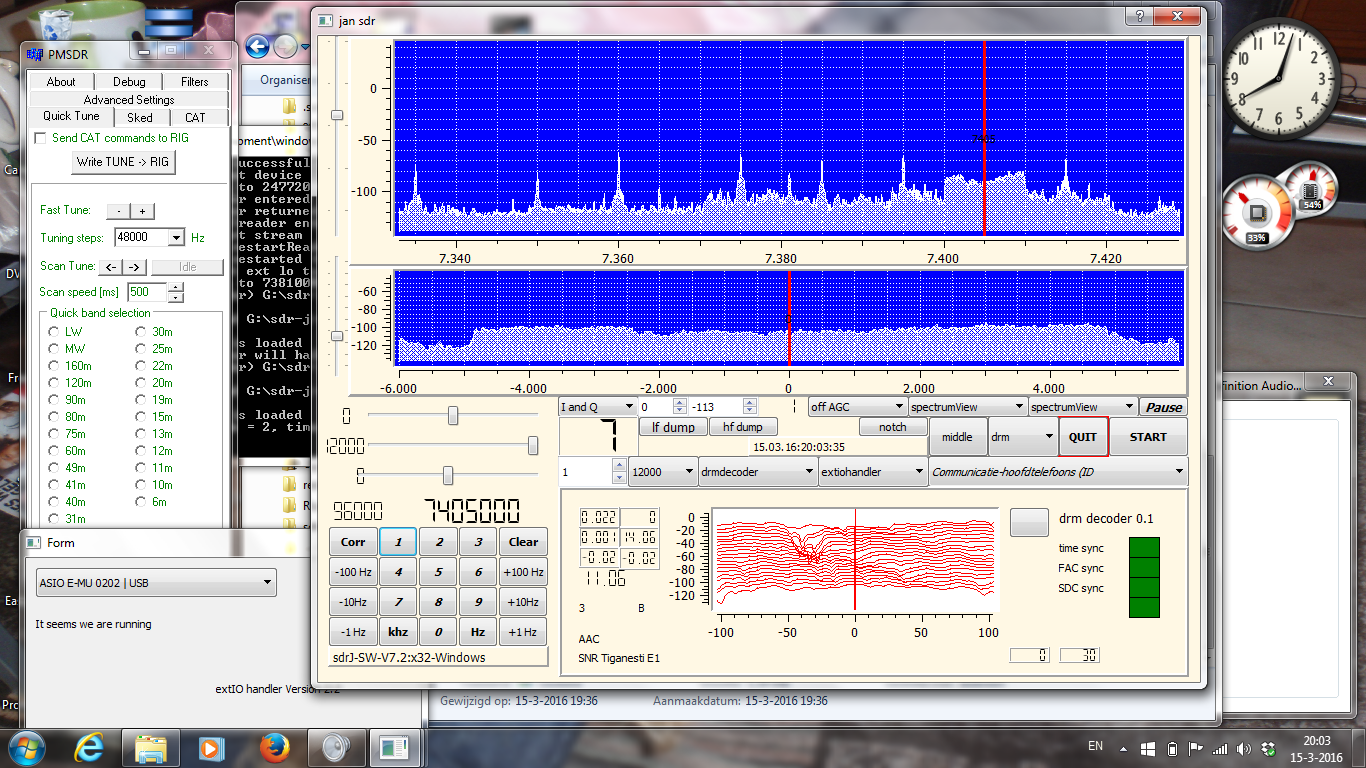
\includegraphics[width=130mm]{Screenshot-extio-pmsdr-sw.png}\footnote{The picture shows
the GUI of the SDR-J sw-receiver while receiving a transmission
from Radio Romania International. OS is Windows 7, input is from a pmSDR and an 
external soundcard EMU 202. Note that some of the other pictures in this
document were made with an older version of the sw-receiver.}
\ \\
\section{Introduction}
DRM is probably not (yet?) the most popular technique
for delivering audio and data over a shortwave radio channel.
Nevertheless, in this time of digital modes for all
kinds of data to be transferred, it is worth investigating.

SDR-J is a (hobby) project in which software for the receiver side
of "SDR", i.e. Software Defined Radio, is being developed.
The developed software set
currenty consists of three  major programs,
a DAB decoder, an FM decoder and a more general (so-called)
shortwave receiver (sw-receiver).

The sw-receiver\cite{swreceiver} 
started as a piece of software to control  - and get some sound from  - the
"Elektor" SDR card \cite{Elektor07},
it developed into a system for other devices as well.

In order to be able to handle a great variety of input devices and
a range of decoders, input controllers  as well as
decoders are implemented as {\em plugins}. Qt, the framework used
for the development, has pretty good support for that.

A dozen decoders was implemented for the sw-receiver,
apart from the - almost obvious - analog usb and lsb decoders,
there are decoders for several other modes, such as rtty, psk, cw, weatherfax,
etc.

Currently
I am using a SDRplay device \cite{sdrPlay} and a pmSDR device \cite{pmSDR}
as  standard input devices for receiving shortwave transmissions under Linux.
For use under Windows, a module is available that provides
support for the "extIO-XXX" \cite{extio} device handlers.
In my environment, both aforementioned devices are well served using the
extio-XXX device handlers.


The software is being developed under Linux and
is cross-compiled for Windows using the Mingw64 toolchain.
It is written in C++, and use is made of the Qt and Qwt libraries
for implementing the GUI. For handling the DFT's we use of
the fftw library\cite{fftw} and support for making sound from the aac samples
is by libfaad\cite{libfaad}. For feeding samples to the soundcard portaudio\cite{portaudio} is used, and for reading and writing ".wav" files libsndfile\cite{libsndfile} is used.
\ \\
The development of a DRM decoder turned out to be more
challenging than expected beforehand, handling OFDM  for DRM
required quite some studying and experimenting.
A  reasonable complete version of the decoder is operational and included
in the 7.x distribution of the sw-receiver.
The version supports audio decoding, and - in a limited form - decoding
of MOT data.

In this paper a very informal description of the implementation
of the {\em synchronization} in the DRM decoder is given, since,
together with the multi-layer decoding of the bits, synchronization in the
receiver is the major challenge\footnote{Once the bits are "in", most work is - from a programmers point of view - straightforward and sometimes even boring}
in the development.

The objective of the paper is to provide some insight in the construction
of the software to ease its comprehension.
After all, the software is open source and for open source
to be successful it is imperative that its sources can be understood.

In section 2 a very brief introduction to OFDM and DRM is given,
in section 3 we briefly discuss the steps involved in mapping the
input samples onto the DRM frames, and we give a - global - overview
of the structure of the front end of the decoder.

In section 4 - the major part of this paper - we discuss the structure of the individual computations
in order to synchronize and equalize.

In section 5 we conclude with some final remarks.

The code of the DRM decoder  is to be found
in the sourcetree at ".../sdr-j-swreceiver/swreceiver/plugins/decoders/drmdecoder".

\section{OFDM and DRM}
\subsection{OFDM}
\ \\
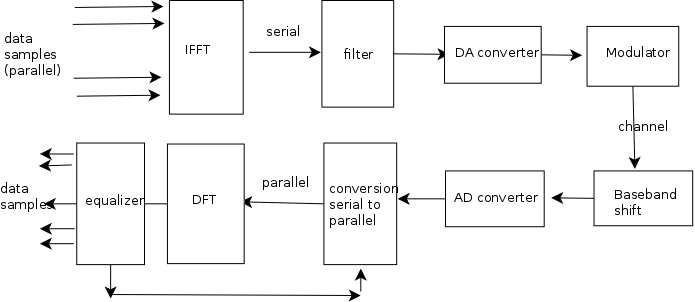
\includegraphics[width=140mm]{ofdm.png}
\ \\
There are many introductions and tutorials on OFDM to be found
on the internet e.g. \cite{ofdm}
A (very) simplified description follows.

The principle of OFDM is pretty straightforward.
Suppose we want to transmit a stream of binary words,
each word containing $N$ bits.
The bits are encoded into complex values (one complex value can be used to
encode up to 6 bits, using both phase and amplitude), resulting
in $M$ complex values for the encoding of the word.

This word with the $M$ complex values is considered to
represent M carrier values in the frequency domain and
is fed into an IFFT device.
The result is a sequence of complex values 
considered to be values in the time domain (symbols), i.e.
the IFFT serialized the input words.

For each resulting symbol in the time domain we copy the
last $Tg$ values and add them
in front of the word (a cyclic prefix) (the value of $Tg$ is one of the
key parameters). This will show to be very helpful
in synchronizing the receiver with the transmitter.

The sequence of (complex) values forming a word this way then is fed into
a DA converter, and the resulting analog signal is
send through some filters and a modulating device.
In a continuous process such words are added
to the input, through the process, to the analog output.

On the receiver side  we transform the received signal into baseband,
and we feed the analog signal into an AD converter to obtain
a sequence of samples.
We extract words of $Tg + M$ samples, and remove in each word
the $Tg$ samples of the
cyclic prefix from the word.
For each word, the remaining samples are then fed into an FFT device.
The result is then words with $M$ complex values.
Due to channel behaviour, the $M$ complex values might suffer from
phase and mplitude errors, however,
after some beautifying
the output (i.e. the equalization) we should have a pretty accurate copy
of the $M$ values that were sent.
We decode
the resulting $M$ complex values from the output to get our $N$ bits back.

The samples of the received analog data should - obviously -
be fully synchronized with the samples in the sending process.
Since - in general - coherent demodulation is used, the data to be
decoded should be an exact copy (both phase and amplitude) of the
data sent. There are many issues in reconstructing the signal, the amount
of papers on topics related to this is impressive.
\subsection{DRM}
DRM is defined in \cite{drm-definition}

A DRM transmission is centered around transmitting
{\em frames} as elements with relevant data.

Each frame is built up from {\em ofdm-symbols},
where an ofdm-symbol - we are in the
frequency domain - can be considered to be built up as an array
 of (complex) carrier values.
The amount of symbols, forming a frame is depending on the mode.

3 frames form together a {\em superframe}. A superframe
contains audio or textual data as well as a full description of how
to interpret and access the data.

Transmission - the time domain - is based on the duration
of a sample of 1/12000 second. 
The duration of transmitting a frame is 400 msec (i.e. it takes 4800 samples),
and a transmission of a whole superframe therefore takes 1200 msec.

The precise structure of a frame is defined by the $robustnessmode$.
DRM supports 4  of such modes, called {\em A, B, C, D}. Different 
robustnessmodes
have different capabilities directed towards particular
transmission conditions.
Robustnessmode $A$ requires stable conditions with very low fading, 
robustnessmode $B$
can handle somewhat more fading conditions etc.

Important parameters are determined by this $robustnessmode$
and the $spectrum-occupancy$. 
\begin{itemize}
\item the number of ofdm-symbols in a frame, e.g.
$robustnessmode$ $B$ (used by transmissions of Radio Romania
International, one of the few
european transmissions using the DRM system) counts 15 ofdm-symbols
in a frame, while $robustnessmode$ $C$ takes 20
ofdm-symbols with less carriers in a frame.
\item The  number of samples, forming a time-domain symbol is
defined by variables $Ts$, $Tu$ and $Tg$ indicating resp.
the number of samples for a full time-domain symbol,
the number of "useful" samples in such a symbol, and the length of the
cyclic prefix (in terms of samples).
For $robustnessmode$s $A$ and $B$ $Ts$ is 320,
the time it takes to transmit
the data of the time-domain symbol is thus $320 * 1 / 12000$ second, the time
to transmit all samples constituing a
frame is $15 * 320 / 12000$ second, i.e. 400 msec.
In $robustnessmode$ $A$ the $Tu$ is 288, in $robustnessmode$ $B$  it is 256.
The length of the cyclic
prefix ($Tg$) is therefore 32 samples in $robustnessmode$ $A$ and 64 in 
$robustnessmode$ $B$. 
\item The number of carriers, depending on the $robustnessmode$ and the
$spectrum-occupancy$.
The $Tu$ samples in the time domain are - using an DFT - transformed into
$Tu$ carriers in the frequency domain.
The outermost carriers do not contain useful data,
the $spectrum-occupancy$ defines which carriers of
these $Tu$ are to be used for data.
As an example, the $Tu$ of robustnessmode $B$ is 256,
with carriers, carrying
useful data, -103 .. 103 in the $spectrum-occupancy$ that is normally used.
\item Pilots. Some carriers (the "pilot" carriers) contain predefined data,
data on known positions in a frame that can be used for
synchronization purposes. The carrier
position and the contents are defined by the $robustnessmode$ and the
$spectrum-occupancy$.
The distance (in number of carriers) between pilot carriers
in an ofdm-symbol is constant.
Pilot patterns differ in subsequent ofdm-symbols,
but the pilot pattern itself is repetitive, i.e. it returns
every X-th ofdm-symbol within a frame.
For e.g. $robustnessmode$ $B$, the distance between successive
pilot carriers in an ofdm-symbol is 6, while the
repetition factor of the pattern
is 3. Since there are 15 ofdm-symbols in a frame in this $robustnessmode$,
each pattern appears 5 times in such a frame
(note however that the  pilot values
on corresponding carriers in different ofdm-symbols may differ).

The basic idea is that for each carrier the channel can be constructed
(and the carrier value reconstructed) by looking at
the values in the pilot carriers as they are appear in the received
signal compared to the values as they should have been.
Next to "regular" pilots, there are several other kinds of pilot:
\begin{itemize}
\item {\em time pilots} appear in the first ofdm-symbol in a frame and will be used
for identifying the first ofdm-symbol in a frame.
\item {\em frequency pilots} appear in all ofdm-symbols on the
same carrier positions,
positions that are defined by the $robustnessmode$.
These frequency pilots may assist in
determining the carrier zero. Once we know which carrier is the real carrier
"zero", we can easily compute the amount of carriers that we are off.
\item {\em boosted pilots} are pilots at carriers at either end of the
ofdm-symbol
with a somewhat higher amplitude than the others.
\end{itemize}
Note that the sets of pilots are not disjoint, i.e. some regular pilots
are also "frequency pilots", and all boosted pilots are regular pilots.
\item Data is organized in three classes:
\begin{itemize}
\item a Fast Access Channel (FAC), data in a set of fixed locations within
each frame that contain data, relevant for the interpretation of the
data in this and other frames. 
The FAC cells are encoded 4QAM (i.e. 2 bits per value)\footnote{for 4QAM
the quadrant the value is in, is determining the 2 bits. For 16QAM each quadrant
houses 4 possible positions, and the value can encode
4 bits determined by phase and amplitude. For 64QAM
each quadrant houses 16 possible positions, and the value can encode 6 bits
determined by phase and amplitude.}
so basically as long as the phase is
more or less correct, correct data can be extracted.
\item a Service Description Channel (SDC), data appearing in the first
few ofdm-symbols of the first frame of a superframe. The data in the SDC
is used to provide additional information on the contents of the superframe.
SDC cells can be encoded in either QAM4 (with 2 bits per value) or
QAM16 (with 4 bits per value),
the encoding is registered in the FAC.
\item a Main Service Channel (MSC). All carriers that are not used
for either FAC,
SDC or pilot are available as data cell for the Main Service Channel.
These data cells may contain sound or text, a description is to be found in the SDC.
MSC cells are encoded as QAM16 or QAM64 (6 bits per value).
\end{itemize}
\end{itemize}

Decoding  of all data items is $coherent$, i.e. for decoding both the phase
and amplitude of the value are important.
It is assumed that
the values contained in the different carriers in the
reconstructed frame resemble the originally values sufficiently
to allow decoding into bits.

Obviously, 4QAM encoded data is not that
sensitive to phase errors or amplitude errors.
16QAM and 64QAM require more precision in the reconstruction of the frames.
\section{From samples to frames: global overview}
\subsection{Introduction}
Once we manage to get the frames identified and filled
with the appropriately restored data values,
extracting bits is pretty straightforward (multi-layer and convolutional
decoding is used).
The main challenge for the DRM decoder is therefore the reconstruction
of the frames.

The first hurdle to overcome is to locate the position of the first
sample in the time-domain inputstream and to detect the 
$robustnessmode$ of the transmission.
Contrary to e.g. DAB, the inputstream does not contain
particular markers between time-domain symbols or frames,
so we need to look at the data itself
to find the start.

Once the location of the first sample of a time-domain symbol in the
inputstream is known, the $robustnessmode$ and the
$spectrum-occupancy$ can be computed and
relevant, mode dependent, parameters, i.e.
the $Tu$, $Tg$ and $Ts$, the number of carriers with useful data,
the pilot positions within
the ofdm-symbols and their pilot values, are known.

Knowing these parameters, processing a samplestream can be viewed
as shifting in $Ts$ samples per time-domain symbol (where $Ts$ is defined
by the robustnessmode of the transmission) into a buffer,
deleting the $Tg$ samples of the cyclic prefix, thus extracting
the $Tu$ samples with useful data, applying a DFT and
$equalizing$ the
data in the ofdm-symbol such that the resulting data is - as good as possible -
a copy of the data transmitted.

Building up a frame requires the identification of the first
ofdm-symbol of this frame,
then collecting the subsequent $symbolsperFrame - 1$
ofdm-symbols, where $symbolsperFrame$  denotes the amount of
symbols in a frame for the mode we are in.
$Time\ pilots$ are helpful with the identification of the first symbol
in a frame.

$Equalization$ will - in general -  require looking at
the values on the pilot positions 
and compute the channels of the pilot positions.
The equalization of the data carriers in a symbol of the frame
then can be done using some form of interpolation of the
transforms for the pilot carriers.

After equalization, the values of the carriers in the ofdm-symbols
in the frame are assumed to
be "exact" copies of the data as sent.

Each complex value of a data carrier then represents a number of bits, depending
on the coding (i.e. 2 bits for QAM4, 4 bits for QAM16 and 6 bits for QAM64).

There are a few things to address though:
\begin{itemize}
\item 
as discussed, the first sample of a time-domain symbol in the input stream
has to be detected;
\item
in general there will be some $frequency\ offset$ in the baseband signal in
the receiver side, sometimes a constant offset by some
offset in the frequency selection, sometimes a varying offset
due to instability of the
oscillator. The frequency offset should be detected and compensated for.
\item
at least as important - we have to ensure that the $time\ offset$ is
compensated for. A time offset  may occur since
\begin{itemize}
\item the  sampling positions  in the  analog signal
do not necessarily coincide with the precise position
the samples had in the
input datastream, i.e. a timing error.
\item the clock used for sampling may not be accurate.
\end{itemize}
\item phaseshifts and amplitude errors due to the channel behaviour
should be compensated for.
\end{itemize}

Frequency as well as time offset errors are really killing the performance,
so spending some additional effort to get that right is really a must.
\subsection{Main flow in the DRM decoder}
In our DRM decoder, frame reconstruction is driven by a mainloop,
continously executed in a separate thread.

In
a schematical form the flow can be depicted as in the picture below.
\ \\
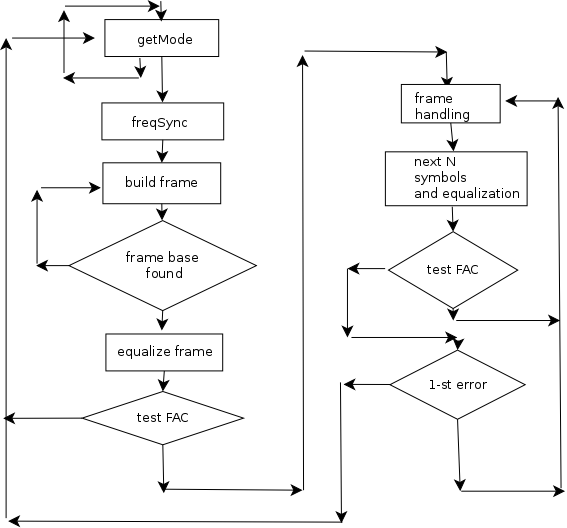
\includegraphics[width=100mm]{flowvoordrm.png}
\ \\
In this picture:
\begin{itemize}
\item the main loop is implemented in the $run$ function in
the class $frameProcessor$.
\item the loop starts with a call to a function $getMode$, member of
the class $Syncer$.  That function
will {\em peek} into the inputstream and
will (try to) compute the robustnessmode, the location of the first
sample of a time-domain symbol in the inputstream,
and - additionally- it will compute a (preliminary) estimate for
the time offset, as well as for
the (fine) frequency offset and the
sampling clock offset. If not successful, the value
-1 is returned.
In the case of no success, the function will skip over
a number of input samples and make a new attempt.
If successful, the input pointer will be set to the first sample
of the time-domain symbol in the inputstream.
\item Once we know where the time-domain symbol starts in the inputstream, we
instantiate a class $ofdmProcessor$. That class
contains functions for reading samples with the given robustnessmode, and
it contains the function $frequencySync$.

When $frequencySync$ is called it will peek into the input
(now starting at the first sample of a time-domain symbol),
and it will compute  the coarse frequency offset, 
an  $integer\ frequency\ offset$, i.e. the frequency offset
expressed in terms of the frequency distance between two successive carriers.
The function will also try to figure out what the $Spectrum-occupancy$ is
by looking at the spectrum.
(Unfortunately, if the $Spectrum-occupancy$ found differs from the default one
some instances of classes have to be deleted and reinstantiated with
the correct class.)
\item 
As soon as the $robustnessmode$ and the $spectrum-occupancy$ are known,
all relevant parameters
can be extracted. We know the $Ts$, $Tu$ and $Tg$ as well as
the number of carriers with useful data and the carrier numbers for the
lowest ($K\_min$) and the highest ($K\_max$)
carrier with useful data, we know the $symbolsinFrame$, i.e. the number
of symbols constituing a frame, and we start reading in 
$symbolsinFrame$ ofdm-symbols by calling "getWord" to fill the buffer $inbank$
with  symbols.
$getWord$, an overloaded member of "frameProcessor"
will read in samples, it will do (time and frequency) adjustments, apply
an FFT and select and reorder the "useful" carriers and make them available.
\item 
We continue reading by calling this function $getWord$ until we
capture a $symbolsinFrame$ symbols, potentially forming a frame.
Since the first (zero-th) ofdm-symbol of the frame
has additional pilot information, checking that we indeed have a full
frame is by looking at $symbolsinFrame - 1$ symbols back and
correlating the samples of the symbol with the time pilots for the given
robustnessmode.
\item We equalize the frame by sending the $symbolsinFrame$ symbols
to a method $equalize$, a member of the class
$Equalizer\_1$\footnote{Many different equalizers were tested,
the number "1" is reminiscent of that}. This equalizer needs to look into
some ofdm-symbols of a next frame before having finished equalizing a frame.
As soon as the equalizer finishes equalizing a frame, the equalized
frame resides in a two dimensional structure  $outbank$,
with values for ofdm-symbol $i$ at $outbank [i]$.
\item ... and we test whether or not we can extract a valid FAC from the frame,
a function $getFACdata$, applied to the frame, will return $true$ is
the FAC data meets the CRC requirements. The function is a member of the
class $frameProcessor$.

If the FAC test fails, we give up and restart.
\item If we do have a valid FAC, it is pretty reasonable to
assume that we have a frame.
We handle the frame (a description of which
is not part of this paper) and interpret the data, e.g. by generating audio
and extracting other data.
\item After having handled the frame, we read in the next N time-domain
symbols, using an overloaded (different) version of $getWord$,
member of  the class $ofdmProcessor$. The function will make new ofdm-symbols
available.
We do the equalization ($equalize$) such that we have a next full frame.
The equalizer will also return $tracking\ values$ for the frequency
offset and for the $time\ offset$ and will recompute the
sampleclock offset, these
values will be used by the version of $getWord$  used in this loop,
to compensate the errors in time and frequency.
\item
Again, the basic validity test is whether or not the frame will have a valid
FAC part. If the frame passes the FAC test ($getFACdata$), we continue our main loop.
\item If, however, the FAC test fails, we won't be too rigid,
if it is the first failure
after a sequence of successes, we just consider it a mistake and continue
our main loop. If it is the second error in a row, we assume a synchronization
failure and give up. 
\end{itemize}
\subsection{Classes}
The following classes are relevant for the synchronization
\begin{itemize}
\item the class $drmDecoder$ is the class managing the interface to
the $sw-receiver$ and handling the local GUI.
It will receive the incoming samples
and put them into the buffer, the latter implemented in the class $simpleBuf$.
\item the class $simpleBuf$ implements the input buffer.
The class has a member function $needed (n)$ that, when called,
will ensure there are "n" samples available. If needed it will wait
until the amount is in the buffer (assuming the client runs in
a separate thread).
\item the class $Syncer$, the home of the $getMode$ function inherits from
the class $simpleBuf$ to ease lookahead in the inputbuffer.
\item the class $ofdmProcessor$ implements the mappers from the samplestream
in the timedomain to the ofdm-symbols in the frequencydomain.
It has three overloaded members $getWord$ and contains the public
member $frequencySync$ and the private member $get\_binZero$.
\item the class $frameProcessor$  implements the main loop,  continously
trying to synchronize on the input and construct frames for data extraction.
It is derived from the class $QThread$.
It has a public member $stop$ that, when called, will set
a variable $isRunning$ to $false$. This variable
will be tested in the main loop.
\item 
the class $Equalizer\_1$ implements the equalizer. For historical reasons 
it is derived from a class $equalizer\_base$.
$Equalizer\_1$ has - apart from
constructors - a single public member, called $equalize$ that - when called -
adds an ofdm-symbol to the equalizer. It returns $true$ when
a frame is synchronized,
and it returns through its parameters tracking values for the
fine $frequency\ offset$,
and $time\ offset$ and it will compute a
new estimate of the sample clock offset.
\item the class $Estimator\_x$ with - apart from the constructors - a
single public member, called $estimate$ that, when presented with
the values of a symbol, will return the channel estimate for the pilot carriers
in that symbol.
In the configuration setting of the current implementation, one may choose
among three implementation for the channel estimation.
\end{itemize}
\section{Computations for the synchronization}
While many of the operations are trivial, 
operations dealing with synchronization,
pretty crucial for successful DRM decoding, are not.
Some of these operations will be discussed in more detail:
\begin{itemize}
\item extracting the $robustnessmode$ and $spectrum-occupancy$
and locating the start
of the symbol in the time domain stream.
\item initial computation of the "coarse" frequency offset for correcting
the VFO, and
\item initial computation of the "fine" frequency offset for correcting
the VFO and the time offset.
\item Once we are in sync and running, the offsets of the fine
frequency offset and time
offset are continuously computed and used for compensation.
\item channel estimation and equalization.
After applying the DFT we equalize the ofdm-symbols, such that we
have the right (or more realistic: best) values for bit decoding.
\end{itemize}
\subsection{Extracting the robustnessmode and locating symbol start}
The robustnessmode can only be detected by looking at the
samples in the time domain inputstream.
The basic idea is to look at correlations:
when we know the location of the first sample of a time-domain symbol,
we also know that the
sum of the correlations of the first $Tg$ samples with the
corresponding samples $Tu$ places ahead is maximal.
This follows directly from the use of the
cyclic prefix, which is (at least at transmission time) an exact copy
of the samples at locations $Tu .. Ts$ within the time-domain symbol.

A first approach then would be to compute the correlation
for a sequence of samples
for a given robustnessmode. If $z$ is the inputstream we compute for
a sample with index $m$:
{
\ \\
$\Phi (m) = abs (\sum_{r=0}^{Tg-1} z_{m + r} \times z_{m + Tu + r}^*)$
\ \\
}
and look for the index $m$ where $\Phi (m)$ is maximal.

In the DRM decoder we apply an MSEE based extension
(from \cite{Tsai}, formula 5.16)\footnote{complex $z_m^2$ is computed as $z_m \times z_m^*$} to compute $\Phi$ for a given index $m$ in the input stream $z$.
{
\ \\
$\Phi_{msse}(m) = \sum_{r=0}^{Tg-1} abs (z_{m+r}^2) + \sum_{r=0}^{Tg-1} abs (z_{m+ Tu + r}^2) - 2 \times abs (\sum_{r=0}^{Tg-1} z_{m+r} z_{m+Tu+r}^*)$
\ \\
}
We then compute 
$\Phi_{msse} (m)$ for $m = k .. k + Ts$ and look for
the $m$ where $\Phi_{msse}(m)$ is minimal ($k$ being the
index of the first available
sample in the inputstream).

Doing so for each of the DRM robustnessmodes considered,
the minimum of the minima 
indicates the  robustnessmode and the index of the first time-domain
sample in the input stream.

\paragraph{Implementation}
The functionality is implemented in the function $getMode$, a member of
the class $Syncer$.
The class extends the class $simpleBuf$ that implements the input buffer,
so from $getMode$ we have direct access to all buffer elements.

$getMode$ computes, apart from the robustnessmode, the index
in the input buffer for a symbol to start, and it computes an
estimate for the fine time offset,
the frequency offset and the sample clock offset.

Implementation is in two parts, in the first part the robustnessmode
is determined,
in the second part, relevant parameters for the mode are computed.

Implementation  of the first part is an almost literal translation of
the formula discussed above.

For each of the DRM robustnessmodes correlations $s [i] \times s [i + Tu]^*$
are computed for the samples $s [i], i \in 0 .. nSamples - Tu$.

Then  $summedCorrelations$ and $summedSquares$ are computed over
the sequence of samples as sum of $Tg$ correlations resp. squares.
{
\ \\
$summedCorrelations = \sum_{i=0}^{nSamples - Tu} s [i] \times s [i + Tu]$
\ \\
}
and
{
\ \\
$summedSquares = \sum_{i=0}^{nSamples - Tu} real (s [i] \times s [i]^* +
                            s[i + Tu] \times s [i + Tu]^*)$
\ \\
}
Furthermore, we compute $Ts$ terms
{
\ \\
$squareTerm[i] = \sum_{j=0}^{nSymbols} 0.5 \times summedSquares [j * Ts + Tg + i]$
\ \\
}
We store the value for the $summedCorrelations$ as $\gamma$.
The minimum value for
the result of $squareTerm [i] - 2 * abs (\gamma [i])$ is determined.
For each of the 4 robustnessmodes this is done, the minimum value indicates the 
mode we were looking for.

A simple "validation" test is looking at the relative value
of the correlation. We assume we are correct when the value
obtained for the the mode found is at least double of the values
for the other modes.

Computing the terms over more than a single symbol in the inputstream
allows us to  give rough estimates of the time offset
and the sample clock offset.

For estimating the $time\ offset$ we take the offsets ($offset_i$)
of the $s$ subsequent symbols that we computed anyway, and apply
a form of averaging\cite{Tsai}:
\ \\
{
$\frac{((\sum_{i=0}^s offset_i) \times (\sum_{i=0}^s i \times i) - \sum_{i=0}^s i * \sum_{i=0}^s i \times offset_i)}{((s - 1) \times \sum_{i=0}^s i \times i - \sum_{i=0}^s i \times \sum_{i=0}^s i)} $
}
\ \\

Computation of the sample clock offset is done by looking at the slope
of the offsets found\cite{Tsai}
\ \\
{
$\frac{((s - 1) \times \sum_{i=0}^s (i \times offset_i) - \sum_{i=0}^s i * \sum_{i=0}^s offset_i)}{((s - 1) \times \sum_{i=0}^s (i \times i) - \sum_{i=0}^s i \times \sum_{i=0}^s i)} \times \frac{1}{Ts}$
}
\ \\

Finally, computation of a first estimate of the fine $frequency\ offset$
is simply by looking
at the phase of the sum of the correlations
{
\ \\
$arg (\gamma [offset_{sample_0}])$
\ \\
}

from which it is easy to derive an estimate for the offset in Hz.
\paragraph{Results}
One shouldn't overrate the quality of the estimation procedure,
estimates are just estimates.
In the tables below we give the results of estimating the robustnessmode
and the start of the first symbol in the inputstream with resp.
5, 15 and 25  time-domain symbols
lookahead (note that 25 time-domain symbols in robustnessmode $A$
or robustnessmode $B$ means 8000 samples, which takes $2/3$ of a second).

The experiment is carried out by running the DRM decoder on a
prerecorded transmission with medium quality reception (i.e. pretty large parts
of the transmission cannot be converted into audio).
After starting the transmission and manually selecting the
subband, the decoder is started.

The first estimate (i.e. "found 1") is obtained looking at the input
at an unknown position. For the subsequent estimates, the buffer pointer
is shifted $Ts / 2$ samples. I.e., iff the first estimate
is accurate, then the next estimates should all be exactly $Ts / 2$,
for the robustnessmode under consideration this means 160 samples.
{\small
\begin{verbatim}
found 1: Mode = 2, time_offset = 288.166687, sampleoff = 0.001563 freqoff = -1.787721
found 2: Mode = 2, time_offset = 158.666687, sampleoff = 0.003125 freqoff = -1.768491
found 3: Mode = 2, time_offset = 162.833313, sampleoff = -0.001563 freqoff = -1.741446
found 4: Mode = 2, time_offset = 157.500000, sampleoff = 0.004688 freqoff = -1.754578
found 5: Mode = 2, time_offset = 162.833313, sampleoff = -0.007812 freqoff = -1.735270
\end{verbatim}
}

Looking at a lookahead of 15 time-domain symbols, we get
{\small
\begin{verbatim}
found 1: Mode = 2, time_offset = 161.208801, sampleoff = -0.000309 freqoff = 0.281117
found 2: Mode = 2, time_offset = 158.450562, sampleoff = 0.000567 freqoff = 0.285227
found 3: Mode = 2, time_offset = 160.384613, sampleoff = 0.000841 freqoff = 0.285681
found 4: Mode = 2, time_offset = 158.791199, sampleoff = 0.001631 freqoff = 0.266741
found 5: Mode = 2, time_offset = 160.615387, sampleoff = 0.001202 freqoff = 0.277272
\end{verbatim}
}

Looking at a lookahead of 25 time-domain symbols, we get
{\small
\begin{verbatim}
found 1: Mode = 2, time_offset = 26.641296, sampleoff = -0.000577 freqoff = -1.728946
found 2: Mode = 2, time_offset = 159.184784, sampleoff = -0.000374 freqoff = -1.728744
found 3: Mode = 2, time_offset = 160.597839, sampleoff = -0.000442 freqoff = -1.726560
found 4: Mode = 2, time_offset = 159.358704, sampleoff = -0.000374 freqoff = -1.728518
found 5: Mode = 2, time_offset = 160.163025, sampleoff = -0.000244 freqoff = -1.728915
\end{verbatim}
}

For a transmission with an excellent reception, we get using
a lookahead of 5 time-domain symbols
{\small
\begin{verbatim}
found 1: Mode = 2, time_offset = 103.166687, sampleoff = 0.001563 freqoff = 0.547337
found 2: Mode = 2, time_offset = 161.000000, sampleoff = 0.000000 freqoff = 0.553580
found 3: Mode = 2, time_offset = 160.000000, sampleoff = 0.000000 freqoff = 0.556413
found 4: Mode = 2, time_offset = 160.000000, sampleoff = 0.000000 freqoff = 0.558379
found 5: Mode = 2, time_offset = 160.000000, sampleoff = 0.000000 freqoff = 0.552505
\end{verbatim}
}

Using  lookead of 15 time-domain symbols we get
{\small
\begin{verbatim}
found 1: Mode = 2, time_offset = 183.824158, sampleoff = -0.000069 freqoff = -1.465193
found 2: Mode = 2, time_offset = 159.329651, sampleoff = 0.000309 freqoff = -1.466084
found 3: Mode = 2, time_offset = 160.175842, sampleoff = 0.000429 freqoff = -1.467475
found 4: Mode = 2, time_offset = 160.175842, sampleoff = 0.000429 freqoff = -1.469134
found 5: Mode = 2, time_offset = 160.175842, sampleoff = 0.000429 freqoff = -1.468285
\end{verbatim}
}

and using a lookahead of  25 time-domain symbols we see
{\small
\begin{verbatim}
found 1: Mode = 2, time_offset = 223.554321, sampleoff = 0.000127 freqoff = 2.689186
found 2: Mode = 2, time_offset = 159.478271, sampleoff = 0.000161 freqoff = 2.689304
found 3: Mode = 2, time_offset = 160.489136, sampleoff = 0.000157 freqoff = 2.689111
found 4: Mode = 2, time_offset = 160.597839, sampleoff = 0.000151 freqoff = 2.690619
found 5: Mode = 2, time_offset = 159.804352, sampleoff = 0.000105 freqoff = 2.690310
\end{verbatim}
}

The numbers do give some confidence in the approach (Note that
any value  X in the range N - 0.5 .. N + 0.5 is considered to
be an integral value N together with a fractional part (X - N)),
most of the values above have an integral part of 160.

An error in the integral estimate of the position will lead
to errors in the FAC decoding and therefore to restarting the process.

\subsection{frequencySync: Computing the coarse frequency offset}
For computing the coarse frequency offset we will use the fact that 
symbols in the frequency pilots carry three pilots with - 
determined by the robustnessmode  -
predefined locations and values.

Given that we know the robustnessmode, and the location
of the first sample of the symbol
in the samplestream, it is easy to read in $Ts$ samples, and take the
FFT of the last $Tu$ samples. By taking a sequence of N of such time-domain
symbols,
adding up the relevant values of the FFT,
we might eliminate some noise and fading effects (recall that frequency pilots
occur in all symbols on the same positions).

Then, if $s$ represents the presumed
positions of carrier $zero$ in the FFT output, the maximum of
{
\ \\
$F (s) = \sum_{n=0}^{Upperbound} \sum_{j=1}^{3} abs (carrier_{n, s + pilot_j}) $
\ \\
}
will give us the carrier $s$ which is most likely the carrier zero. 
{\em Upperbound} indicates the number of ofdm-symbols 
used in the summation, in the implementation we use the number of
ofdm-symbols in frames of this mode as upperbound.

Given that the (complex) samples in our implementation are taken at 12K,
and given that the bandwidth of the signal can be 10K, it is obvious that
the frequency range we look into is limited. Frequency errors of app
more than 700 Hz are beyond (automatic) correction. Since, however,
the user has a large screen, showing a.o. the spectrum, he is able
to do some coarse correction by himself\footnote{Although too large an offset
cannot be compensated for automatically, the offset is shown on the screen
and can be corrected manually}.

\paragraph{Implementation}
The function $frequencySync$ is implemented as member of
the class $ofdmProcessor$.
It calls upon the function $getoffsint$ to actually compute the frequency
offset and it will estimate the Spectrum-occupancy.

At first it will ensure that sufficient data for $N$ ofdm-symbols
(+ some more) are
available in the input buffer. Next, it will call upon a private version
of $getWord$ to actually read in $N\_symbols$ time-domain symbols
and transform these into $N\_symbols$ ofdm-symbols.

The version of $getWord$ is private a.o. since it only peeks into
the input stream and will not change the buffer pointer for the inputstream.

The function $get\_zeroBin$ will - using the data read in
into the $symbolBuffer$ - decide where the carrier "zero" is, i.e. determine
the frequency offset. The result is a binNumber in the range -Tu / 2 .. Tu / 2.

Spectrum-occupancy is estimated by peeking into a number
of carrier positions (the implementation is a rewrite of the one in
the software from \cite{Bos}).
For the computation, the $binNumber$ is translated
into a number in the range 0 .. Tu.

For each of the possible spectra we identify the minimum and the
maximum of the carriers with useful data (which follows from the $K\_min$
and $K\_max$ for the combination of the $robustnessmode$ and the
$spectrum-occupancy$ we are looking at) for each
of the spectra possible, and we
look at carrier values nearby the edges inside and outside the 
relevant parts of the spectrum
under consideration.

We compute the (relative) energy by comparing the energy 
within a $bin$ that is supposed to be just inside the relevant
part of the spectrum with the energy 
within a bin supposed to be (just) outside that part of the spectrum.

The maximum of the measured values indicates the Spectrum-occupancy.

\paragraph{$get\_zeroBin$}
The function $get\_zeroBin$ will decide which $bin$ in the collected
ofdm-symbols
that are stored in $symbolBuffer$ represents the carrier zero.

A viable alternative to looking at the energy in the bins
is to make use of the strong correlation that exists between frequency
pilots in successive ofdm-symbols vs the correlation between random values.

Computing $K (n, s)$ for symbol $n$ ($n > 0$) in the symbolBuffer, and
for carrier $s$ that are candidate carrier zero.
{
\ \\
$K (n, s) = abs (\sum_{j=1}^{3} carrier_{n, s + pilot_j} \times carrier_{n -1, s + pilot_j}^*) $
\ \\
}

where $pilot_j$ indicates the index for the carrier of j-th frequency pilot.
Extended over the whole symbolBuffer this reads
{
\ \\
$F (s) = \sum_{n=1}^{nSymbols} abs (\sum_{j=1}^{3} carrier_{n, s + pilot_j} \times carrier_{n -1, s + pilot_j}^*) $
\ \\
}

The value $F (s)$ for carriers $s$ in the range $-Tu / 10 .. Tu / 10$  is
computed, the $s$  for which the value is maximal gives the bin number.
This bin number is returned.

\subsubsection{Results}
The computations - with energy levels in the bins in computing
the maximum, or with correlations in computing the maximum -
depend on the quality if the signal,
there is no garantee that in all cases the right bin
is designated the bin representing carrier zero.

\subsection{Initial estimation of time and frequency offset}
As long as we are not synchronized, we have to use time domain data
to estimate time and frequency offset.
It is assumed that the integer frequency offset is stable, i.e. we
do not need to recompute it (obviously until needed).

As long as we are {\em not} synchronized, an overloaded version of $getWord$
is used to read in time domain samples and extract ofdm-symbols,
applying time domain and frequency domain corrections on the input.
\subsubsection{Time offset}
As mentioned above, determining the Robstnessmode has - as a by-product - an
estimate of the time offset. Since it is pretty hopeless to
estimate time offset using only a single ofdm-symbol,
we use the rough estimate
from the robustness detection.
For each symbol read, we adjust the time offset
{
\ \\
$timeoffset_{symbol} += Ts \times timeoffset_{sample}$
\ \\
}
{\em Compensating} the time offset is  done simply by linear interpolation
(the time offset is smaller than half the time between two successive samples).
\subsubsection{Fine frequency offset}
In case the frequency offset is 0.0,
there will be no phase difference between
the samples in the cyclic prefix and the corresponding samples in the
data segment, i.e.
{
\ \\
$ \forall i \in 0 .. Tg.  arg (s [i] \times s [Tu + i]^*) = 0$
\ \\
}
In case of a non-zero fine frequency offset,
the correlation between the time-domain sample
and the conjunct of its corresponding element in the data segment
{
\ \\
$arg (s [i] \times s [Tu + i]^*) \neq 0$.
\ \\
}
The corner itself is a reasonable indicator
for the VFO offset.

By using more than a single pair of samples and averaging the value,
we eliminate some undesired effects
coming from noise. I.e. the fine frequency offset is computed from
{
\ \\
$vfo_{offset} = \frac {arg (\sum_{i=0}^{Tg - 1} s [i] \times s [Tu + i]^*)}{(2 \times \pi)} \times \frac{Samplerate}{Tu}$
\ \\
}
{\em Compensating} the frequency error in the inputstream is
done in the time domain:
a table driven "local oscillator" with a granularity of 0.01 Hz (i.e.
a table with $12000 \times 100$ elements) is used,
and all samples are mixed with values from this oscillator.
{
\ \\
$theAngle = 0.9 \times theAngle + 0.1 \times vfo_{offset}$
\ \\
$theOffset = \frac{theAngle * 1200000}{2 * \pi * Tu}$
\ \\
}

the result is used in the local oscillator to adjust the
VFO frequency in the
time domain.
\paragraph{Implementation}
The implementation of the  computation of the
fine frequency offset and the correction on the
time-domain samples is in the function $getWord$,
member of the class $ofdmProcessor$. 
\subsection{Identifying the start of a frame}
To assist in locating a frame in DRM, the zero-th ofdm-symbol of a frame
contains a pretty large number of additional pilots, the {\em time} pilots.
Identification of the beginning, i.e. locating
the zero-th time-domain symbol of the frame
takes place in the $run$ function - implementing the thread - in the class
$frameProcessor$. 
It is simply done by locating the
symbol with the maximum correlation in a frame.

We compute
{
\ \\
$\forall k \in 0 .. symbolsinFrame\ S(k) = \sum_{i = first}^{last} carrier_{k, pilot_i} \times table_{Mode, i}^*$
\ \\
}

for the last N  odfm-symbols read, and return $true$ if 
$S_0$ is maximal. Note that all symbols of the frame are read alreay,
so the full frame is available.
(It is assumed that $carrier_{k, pilot_i}$ indicates the value
of the carrier of the $i-th$ pilot in the $k-th$ symbol,
and $table$ is an array containing
the time pilot values  for the various robustnessmodes in an ordered way)

Once the ofdm-symbol "zero" is detected, we feed the frame - ofdm-symbol
by ofdm-symbol -
to the equalizer and, after having an "equalized" frame, we
verify that the data in the FAC is valid.
\paragraph{Implementation}
The correlation
{
\ \\
$S(k) = \sum_{i = first}^{last} carrier_{k, pilot_i} \times table_{Mode, i}^*$
\ \\
}

is implemented in a function $getCorr$, private to the class $ofdmProcessor$.

As long as we are $not$ synchronized, the correlation
is computed and stored in a
row of $symbolsinFrame$ elements.
\subsection{Tracking the fine frequency and time offset}
Once we have reasonable values for the parameters and we are in sync, i.e.
the FAC values make sense,
we will use the information extracted from the ofdm-symbols to compute
tracking values for the time and frequency offset.
Leading principle here is
\begin{itemize}
\item a {\em frequency offset} leads to phase offsets in carriers with
the same index in subsequent symbols,
while
\item a {\em time offset} leads to phase offsets in carriers with
increasing indices within the same symbol.
\end{itemize}
As a consequence, the computation of a tracking value for the frequency offset
requires looking at more than a single symbol, while for the 
computation of the  tracking value for the time offset, we can just look
at the most recent one.

Computing the tracking values is done in the function $equalize$, member
of the class $Equalizer\_1$. The input to that function is a symbol
in the frequency domain, its output indicates whether or not a complete
frame was equalized or not.
Through it parameters  the function return three values:
\begin{itemize}
\item an estimate of the error in the fractional time offset,
\item an estimate of the fine (i.e. fractional) frequency offset, and
\item an estimate of the sample clock offset.
\end{itemize}
These values, when computed, are handed over to an (overloaded
version of the) function $getWord$ in the class $ofdmProcessor$.

As long as we are synchronized, the loop in the $run$ function in the
class $frameProcessor$ contains a sequence in which
$getWord$ and $equalize$ are called one after the other.
\subsubsection{Tracking the fine frequency offset}
All ofdm-symbols in a DRM frame carry three frequency pilot carriers,
it is therefore
tempting to use the phase difference between corresponding
frequency pilots in subsequent
symbols as basis for etimating the fine frequency offset. 

On the other hand, there is a repetitive pilot pattern within the ofdm-symbols
in a frame, i.e. each
pilot pattern reappears after a number (defined by the parameters of the
robustnessmode) ofdm-symbols. Since there are far more regular pilots
in an ofdm-symbol than frequency pilots, we can also base the
computation of the tracking value of the fine frequency offset 
on  a comparison of the data using full pilot patterns.
We look at 
{
\ \\
$\delta_f = \sum_{j=0}^{J - 1}\frac{\theta_j}{(2 \times \pi \times \frac{Ts}{Tu} \times J \times d)}$
\ \\
}
where the $\theta_j$ indicates the phase difference - due to a VFO offset -
of pilots at the same positions in two ofdm-symbols with distance $d$. $J$ is
the number of pilots in the symbol. $\theta_j$ is the phase difference:
{
\ \\
$\theta_j = arg (Z_{k, j} \times Z_{k - d, j}^*)$
\ \\
}
where
{
\ \\
$Z_{k, j} = carrier_{k, j} \times pilotValue_{k, j}^*$.
\ \\
}
i.e. the correlation between the value that we got with the value
that it should be (Note that while the pattern of the pilot will repeat
itself, the pilot values for pilots on corresponding positions
in different symbols will be different).

Alternatively, as stated earlier, we could be using the
phase difference between
corresponding frequency pilots in subsequent ofdm-symbols to
compute an average
offset (expressed as angle).
{
\ \\
$\delta_f = \frac{\sum_{k=0}^{3} \frac{arg (\sum_{j=1}^{N - 1} \theta_{j, k})}{N - 1})}{3}$
\ \\
}
where
{
\ \\
$\theta_{j, k} = carrier_{j, freqPilot_k} \times carrier_{j - 1, freqPilot_k}^* $
\ \\
}

\paragraph{Implementation}
Estimation of the offsets is done in the function $equalize$, member of the
class $Equalizer\_1$. The implementation of the two alternatives
results in setting a value for "offs1" and "offs7". One of these,
depending on the setting of the comments, is given back as output.

{\em Correction} of the detected offset is done in the function $getWord$,
an overloaded member of the class $ofdmProcessor$.
Correction is done by adding (a fraction of) the error value
to the frequency corrector, i.e.
{
\ \\
$theAngle = theAngle + 0.1 \times delta_f$,
\ \\
}
and computing the term with which the VFO (in steps of 0.01Hz) needs to
be corrected
{
\ \\
$offset = \frac{theAngle \times 1200000}{(2 \times \pi \times Tu}$ 
\ \\
}

\paragraph{Results}
We ran some tests to look at the differences in computed angles when
using different methods.
The first table shows the differences in the computed offset (in Hz)
when using correlation of the time domain samples (column "initial")
compared to computing a tracking value
using the correlation between corresponding pilots in different ofdm-symbols.
{\small
\begin{verbatim}
found 1: Mode = 2, time_offset = 155.186829, sampleoff = 0.000343 freqoff = -1.035243
......
initial -> -7.610438, tracking -> -6.872640, error -0.069466
initial -> -7.647318, tracking -> -6.869167, error 0.064016
initial -> -7.655280, tracking -> -6.872368, error -0.193599
initial -> -7.656196, tracking -> -6.862688, error 0.036547
initial -> -7.622445, tracking -> -6.864515, error 0.071519
initial -> -7.605674, tracking -> -6.868091, error 0.027857
initial -> -7.661390, tracking -> -6.869484, error 0.102430
initial -> -7.726436, tracking -> -6.874605, error 0.028973
initial -> -7.810171, tracking -> -6.876053, error -0.003366
initial -> -7.804359, tracking -> -6.875885, error 0.080864
initial -> -7.833959, tracking -> -6.879929, error -0.056720
initial -> -7.848853, tracking -> -6.877092, error 0.080997
initial -> -7.853055, tracking -> -6.881142, error 0.061169
initial -> -7.737529, tracking -> -6.884200, error 0.001444
initial -> -7.687623, tracking -> -6.884273, error 0.067440
initial -> -7.696682, tracking -> -6.887645, error 0.019243
\end{verbatim}
}
It shows that the average difference is app 0.8 Hz, for this transmission
the distance (in Hz) between carriers is 46.875, 0.8 Hz is less than 2\%.

The second table shows the - relative - differences between
frequency offsets computed by different approaches.
The "freq pilots" column contains the tracking values using the frequency pilots
of the last $symbolsinFrame$ ofdm-symbols, the column "all pilots" contains
the values when using the phase differences between corresponding
pilot carriers in successive symbols with the same pilot layout.
{\small
\begin{verbatim}
found 1: Mode = 3, time_offset = 81.345032, sampleoff = 0.000021 freqoff = 2.722603
freq error: freq pilots = -0.001238, all pilots  = -0.022117
freq error: freq pilots = -0.002598, all pilots  = -0.029494
freq error: freq pilots = -0.007710, all pilots  = -0.068261
freq error: freq pilots = -0.004116, all pilots  = -0.067595
freq error: freq pilots = -0.010344, all pilots  = -0.071337
freq error: freq pilots =  0.009163, all pilots  = -0.033330
freq error: freq pilots = -0.003729, all pilots  = -0.054826
freq error: freq pilots = -0.006766, all pilots  = -0.071762
\end{verbatim}
}
However, the tracking mechanism ensures that integrating the error
- computed through looking at the phase differences of frequency pilots
in subsequent symbols -
into a freqency offset shows reasonable results.
{\small
\begin{verbatim}
found 1: Mode = 2, time_offset = 277.505493, sampleoff = 0.000137 freqoff = 0.366356
.........................
initial -> 2.772697, tracking -> 1.887462, error -0.015296
initial -> 2.774176, tracking -> 1.888227, error 0.000799
initial -> 2.776244, tracking -> 1.888187, error -0.005090
initial -> 2.753825, tracking -> 1.888442, error -0.010391
initial -> 2.768445, tracking -> 1.888961, error 0.007719
initial -> 2.774968, tracking -> 1.888575, error 0.006177
initial -> 2.763738, tracking -> 1.888267, error -0.002878
initial -> 2.761683, tracking -> 1.888410, error -0.002655
initial -> 2.757870, tracking -> 1.888543, error -0.005434
initial -> 2.768815, tracking -> 1.888815, error 0.005062
\end{verbatim}
}
Again, the differences are less than 2\%.

The measurements were taken using the same recording of a transmission.

\subsubsection{Tracking the time offset}
The effect of a timing error in sampling will be a phase shift over 
carriers with an increasing index within an ofdm-symbol.
This phase shift is therefore an indicator for the time shift.
Since successive carriers are uncorrelated, we need to fall back on successive
pilot carriers within a symbol.
We then look at the difference of the deviations of the phase at the
pilot locations compared to the corresponding predefined pilot values.
We compute for the most recent ofdm-symbol S,
\ \\
{
$time_{offset} = arg (\sum_{j=1}^{j=J} (carrier_{S, pilot_j} \times pilotValue_{S, pilot_j}^*) \times (carrier_{S,pilot_{j - 1}} \times pilotValue_{S, pilot_{j - 1}}^*)^*)$
}
\ \\
The basic assumption here is that the channel $H_{n, pilot_j}$ is
roughly equal to the $H_{n, pilot_{j - 1}}$ which might be the case
in a slow fading environment when the distance - in number
of carriers - between successive pilots is small
(see e.g. \cite{Chang} for a proof).
For robustnessmode $B$, the distance is 6, the results
seem to be good. Even for robustnessmode $A$,
where between successive pilotcarriers in an ofdm-symbol is 20,
the results
are acceptable (note that robustnessmode $A$ is meant for (almost)
fading free transmissions).

\ \\
While computing the tracking values, we also compute an estimate of
the sampling clock offset, using \cite{Tsai} formula 5.40
{
\ \\
$delta_{sc} = \frac{\sum_{j=0}^{J-1} \theta_j \alpha_j}{(2 \pi \frac{Ts}{Tu})(\sum_{j=0}^{J-1} \alpha_j^*)}$
\ \\
}
where $\alpha_i$ is the index of the $i_th$ pilot.
\paragraph{Implementation}
The current time tracking value, is computed in the function
$equalize$, member of the class $Equalizer\_1$. The offset is
computed in a variable $offs2$ and returned through a parameter.

The estimate of the sample clock offset is computed in the variable $offsa$,
and returned through a parameter.

{\em Compensation} of the detected offset is in the function $getWord$,
member of the class $ofdmProcessor$.
Compensation is done by computing an offset value
as the sum of the previous offset value with (a fraction of) the error, i.e.
{
\ \\
$timeOffset = timeOffset + 0.5 \times time_{offset}$
\ \\
}
{\em Correction} of the samples is by linear interpolation.
Although it seems reasonable
to expect that the $delta_{sc}$ can be used to reduce the timing error
between successive samples, however, up until now no
noticeable improvements showed.
\paragraph{Results}
Computing the time offset using the time domain symbols was
tried 
by looking at the phase differences between the correlations of the
cyclic prefix samples with the corresponding samples in the useful part.
Results were disappointing. During the time that we are
not (yet) synchronized, we use - as mentioned before - the time
offset as computed by the $getMode$ function, for each subsequent
symbol adapted by the expected time shift caused by the sample clock offset.

There is a potential discontinuity 
when switching to the mainloop: the first time offset value
maybe a little off, such that FAC (i.e. QAM4) demodulation can be done
but the offsets are too much for reconstructing the QAM16 and QAM64
values.
Computing an accurate time offset with time domain symbols is a topic
for further study and experimentation.

The "quality" of the tracking of the time offset  and the
corresponding correction of the actual time offset can be deduced
from the  computed values for the time offset.
{\small
\begin{verbatim}
found 1: Mode = 3, time_offset = 91.789490, sampleoff = -0.000060 freqoff = -2.475263
time err = 0.000000, clock offset = 0.000000, correction value = 0.208478
time err = 0.001337, clock offset = -0.000015, correction value = 0.207810
time err = 0.000859, clock offset = -0.000033, correction value = 0.207380
time err = 0.002041, clock offset = -0.000045, correction value = 0.206360
time err = 0.001852, clock offset = -0.000053, correction value = 0.205434
...............................
time err = 0.001944, clock offset = 0.000078, correction value = 0.175560
time err = 0.002364, clock offset = 0.000081, correction value = 0.174378
time err = 0.002139, clock offset = 0.000083, correction value = 0.173309
time err = 0.002788, clock offset = 0.000086, correction value = 0.171914
time err = 0.001835, clock offset = 0.000088, correction value = 0.170997
time err = 0.001459, clock offset = 0.000089, correction value = 0.170267
\end{verbatim}
}

The table - derived from measurements on a recording - of radio Nigeria
(Abidja) with robustnessmode C - shows the timing error, and the resulting timing offset.
The time error remains reasonably small, the correction
remains reasonably stable. 

\subsection{Equalization}
The final step in the re-creation of the carrier values in the DRM frames,
i.e. before decoding the bits,
is the equalization, i.e. undoing all kinds of channel effects, such
that the carriers in the frame resemble the carriers as they were sent.

A first - naive - approach of the equalizer was to
compute the channels for the
pilots with a simple algorithm, and apply - symbol per symbol -
simple interpolation to create estimates of the channels
for the other carriers and equalize them.

Algorithms for MLE and MSSE approaches to compute an "optimal" channel
for the pilots exist. We experimented with 
one dimensional algoritms given in e.g. \cite{Morelli}.
The results, combined with a variety
of interpolation approaches, such as sync, fft etc - were somewhat
disappointing, primarily due to issues around {\em extrapolation}. 
Extrapolation was needed to get
estimates of the channels for the outermost carriers, outside the
range of pilot carriers, in the symbols. 

In diorama\cite{Diorama} an equalization algorithm is used that is based on
a two dimensional approach\cite{Wiener}.
Furthermore, the RXAMADRM software made by \cite{Bos}
contains a translitteration
of the Diorama Matlab code in C++ code.
That code was adopted as a basis for rewriting
the equalizer module in the DRM decoder.
\ \\
The basic idea for this kind of equalizer is
to define for each carrier in a symbol a computation
with which an estimate of the channel of that carrier is computed.
The channel for that carrier is then computed by
applying the computation to the pilot channels
of the symbol the carrier is on and using the pilot channels on
the symbols "not too far away" from the symbol the carrier is on.

Pilot channels themselves are easily estimated by comparing
the received value with the value they should have. In our implementation
we default to the simple one, i.e. a quotient of the observed value and the
predefined value\footnote{In the implementation there is the possibility
- a configuration option - for computing the channels of the pilots
using MLE techniques as mentioned in \cite{Morelli}}.

\begin{figure}[ht]
\begin{center}
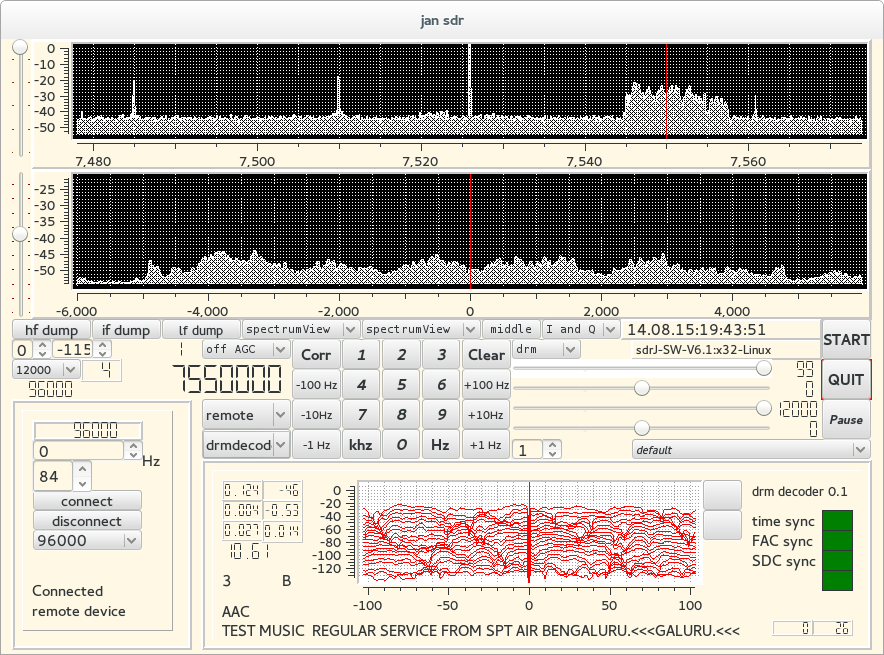
\includegraphics[width=140mm]{screenshot-3.png}
\caption{Amplitude correction by equalizer (2 "spaghetti" lines per frame)}
\label{fig:equalizer}
\end{center}
\end{figure}

Shortwave - where the DRM programs are transmitted - suffers from
severe fading conditions. Figure \ref{fig:equalizer} shows - with the
red lines in the box in the bottom half - the amplitude
correction computed by the equalizer for a sequence of frames.
Each line (two lines from each frame are depicted) in that
picture indicates the amplitude correction 
to be applied to the carriers in a symbol of a frame.

We compute the channel for a given carrier $carrier$ in
a given ofdm-symbol $symbol$ as
{
\ \\
$channel_{symbol, carrier} = \sum_{p \in pilots} channel_{pilot(p)} \times W\_symbol\_blk_{symbol, carrier} (p)$
\ \\
}
i.e. a convolution of pilot values "nearby" the carrier under consideration
with a set of precomputed values.
In the above formula, $pilots$ indicates the set of
pilots of all ofdm-symbols taken
into account (i.e. the pilots "nearby"),
and $channel_{pilot(p)}$ denotes the channel value for  the p-th $pilot (p)$
in this set.

$W\_symbol\_blk_{symbol, carrier} (p)$ denotes the  p-th element of the
predefined values for convolving with the $p-th$ real pilot value
used for computating the channel for carrier $carrier$ in
symbol $symbol$. 

$Equalization$, i.e. restoring the carrier value, is then straightforward,
{
\ \\
$\frac{actualValue_{symbol, channel}}{channel_{symbol, carrier}}$.
\ \\
}
\paragraph{Computing $W\_symbol\_blk$}
It is important to realize that the
pilot pattern repeats itself, after $periodicity$ symbols
pilots are found on the same carrier
positions\footnote{Not taking into account the
additional pilots for "special purposes" in symbol 0.},
however, the pilot values on corresponding positions in
different symbols may differ.

The value of $periodicity$
depends on the robustnessmode,
for e.g. mode A, the periodicity is 5, for mode B
it is 3, for mode C it is 2.

In the approach taken, the computation of the channel for a carrier $c$
in ofdm-symbol $s$ depends on
the pilot values in the symbols $s - a + 1 .. s + a$
(where $a$ is essentially user defined).
We use the term {\em Window} for such a range of $2 \times a$ symbols.
The symbol $s$ is then the base symbol of that Window.

It is obvious that there are only $periodicity$ different windows in 
frames of a given mode (not taking into account different pilot values
on corresponding positions in different symbols within a frame).

Given that there are $periodicity$ different windows in a frame,
it will be obvious that - apart from the particular parameter values -
the computation of the channels in $symbol_i$ is the same as the
computation of the channels in $symbol_{i + k * periodicity}$, for
\ \\
$i + k * periodicity < numberofSymbols (mode)$.
\ \\
$W\_symbol\_blk$ will be implemented as a matrix,
with dimensions ($Windows \times carriers \times pilots\_per\_window$).
\begin{itemize}
\item The first dimension is the number of Windows, i.e. $periodicity$,
indices have 
a value in the range $0 .. periodicity$,
\item The second index indicated the order number of the carrier in 
the base symbol of the window,
\item the third index gives access to a vector with
coefficients for convolving with the real pilot channels.
The number of pilots in the different windows may differ.
\end{itemize}
With such a matrix, computation of the channel for a carrier $c$ in a symbol $s$
is simple:
{
\ \\
$\sum_{i=0}^{NumberofPilots (W (s))} W\_symbol\_blk[W (s)][c][i] *
	           pilotValue_{realAddress [s][Table[W (s)][i]]}$
\ \\
}
In this formula:
\begin{itemize}
\item $W (s)$ is the mapping from the actual symbol to a window;
\item $NumberofPilots (x)$ gives the number of pilots in Window x;
\item $Table [x][y]$ gives the address of the y-th pilot in window x, i.e
an address relative to the first carrier of the first symbol of that window;
\item $realAddress [s][y]$  gives the real address, i.e. $symbol$, $carrier$,
of the y-th pilot in window x, applied on symbol $s$.
\end{itemize}

Following \cite{Wiener}, computing the coefficients requires computing the
cross covariance matrix $\Theta$ and the autocovariance $\Phi$.
Given the $\Theta$ and the $\Phi$, we compute for each window $W$
and each carrier $c$ in the base symbol of that window
\ \\
{
$W\_symbol\_blk_{w, c, pilot} = \sum_{k \in pilots_{w}} \Theta_{w, c, k} \times \Phi_{k, pilot}^{-1}$
}
\ \\
with
\ \\
{
$\Theta_{w, c, pilot} = sinc ((c - carrier_{pilot}) \times f_{cut_k}) \times sinc ((periodicity / 2 - symbol_{pilot}) \times f_{cut_t})$
}
\ \\
where $pilots_{window}$ denotes the set of pilot locations
(each pilot addressed as (symbol, carrier)),
$carrier_{pilot}$ indicates the  ($symbol$, $carrier$) position of the pilot,
$periodicity$ indicates the afore mentioned
periodicity of the pilot patterns in the symbol, $symbol$ is the (relative)
number of the symbol carrying the pilot.
\ \\
$f_{cut_t}$
is an estimate
for the two-sided maximum doppler frequency (normalized w.r.t.
symbol duration Ts), and
\ \\
$f_{cut_k}$
is an estimate for the
two-sided maximum echo delay (normalized w.r.t useful symbol
duration Tu).
\ \\
$\Phi$ is computed over all regular pilots appearing in a window, and is
- per window - a 2-dimensional array, with:
\ \\
{
$\Phi (pilot_1, pilot_2) = sinc ((carrier_{pilot_1} - carrier_{pilot_2}) \times f_{cut_k}) \times
sinc ((symbol_{pilot_1} - symbol_{pilot_2}) \times f_{cut_t})$
}
\ \\
$carrier_{pilot_i}$ indicates the carrierposition of $pilot_i$.
$symbol_{pilot_i}$ indicates the (relative) ofdm-symbol number where the pilot
resides (relative to the first symbol of the window we are dealing with).

\paragraph{Implementation}
The implementation in a class $Equalizer\_1$ follows the outline given above. 
The constructor of the class will precompute 
$W\_symbol\_blk$ along the lines, mentioned above.

The quality of the equalization depends (a.o) on the size of the windows.
Since the amount of pilots used in the computation
depends on the window size, larger windows mean
more computations per element. 
To experiment, one of a couple of different sizes for
the windows (i.e. the number of symbols for which
the pilots are used in the window) can be selected.
Selection is through a setting in the ".ini" file.

Values
$f_{cut_k} = 0.0675 \times \frac{1}{windows}$ and
$f_{cut_t} = 1.75 \times \frac{Tg}{Tu}$
are taken from \cite{Diorama} and
adapted for minimal disturbance of the equalizers (i.e. different procedure
for different robustnessmodes).

The actual estimators used for estimating the channel values of
the pilots are selected by a configuration parameter,
the trivial one does not need additional matrix operations, the MLE based
ones require the armadillo library\cite{armadillo} for the
matrix operations involved. By default the trivial one is selected\footnote{It is obvious that lots of experiments were done with the other approaches as well, however, differences is performance were not noticeable}
\ \\
$channel_{pilot_j} = \frac{actualValue_{pilot_j}}{definedValue_{pilot_j}}$
\ \\
The estimators are implemented in instances of a separate
$Estimator\_1$ class.

For each window $W$ the - relative - locations of the pilots in the window
are computed by the function $buildTrainers$. The locations
of the trainers (addressed as pair (symbol, carrier) are stored
in a vector, addressable through $theTrainers [window]$.
Once these "trainers" are built, for each window
the $\Phi$ matrix is computed as indicated above in nested loops.

In the same loop for each carrier the $\Theta$ is computed -
again the implementation follows the description above -
and for that carrier $c$
the vector $W\_symbol\_blk [W][c]$ is computed.

The actual equalization for a carrier then
takes as steps:
\begin{itemize}
\item identifying the vector in $W\_symbol\_blk$ that is applicable 
for the carrier;
\item convolving the actual pilot values of the window under consideration
with the the value (a vector) of $W\_symbol\_blk$ to obtain the
channel for the carrier under consideration.
\item applying the channel value to equalize the carrier.
\end{itemize}
Note that the channel values are stored; they are used in the symbol decoding 
later on.

The vector to be equalized
is placed in the $Frame$,
computations for tracking values are done, and
- within the function $processSymbol$, the actual 
computation is done (using the channel values on the pilot locations).

The result is stored in a row in the two-dimensional array $outFrame$.

\section{Final remarks}
In order to get a better understanding of the structure of DRM,
both the Matlab code of
Diorama\cite{Diorama} and the C++ translitteration of Diorama in C++
as done in RXAMADRM \cite{Bos}
were looked at. Both proved to be a great help.
Some parts of the DRM decoder
are a rewrite of the C++ code in  RXAMADRM, other parts were
- at least - inspired by Diorama and RXAMDRM.

The SDR-J software uses a number of libraries, made available
through (L)GPL style licenses and parts of the code is
based on ideas of others.
In all cases attempts are made to indicate the rightfull
owner of the copyrights. The software itself is available ”as is”,
under a GPL V2 license.

The SDR-J software is a hobby project, its development is neither
driven by time constraints nor deadlines, but purely by curiosity.
It allows to re-implementations of sections, something
that has been dome regularly.
The software is - obviously - not finished, after all
it is software and as far as I am concerned, it never will be finished.
Many enhancements (and experiments) are still waiting to be done.
Support in any form - suggestions, code improvements or donations - is
always welcome.
\begin{thebibliography}{9}
%
\bibitem{swreceiver}
Jan van Katwijk,
SDR-J-SW-7.1,
Software for SDR : The 32 bits SW receiver,
see "http://www.sdr-j.tk"
%
\bibitem{Elektor07}
Burkhard Kainka,
Software Defined Radio
Met USB-interface,
Elektor 5/2007.
%
\bibitem{extio}
Alberto, I2PHD,
Winrad - specifications for the external I/O DLL,
Document found on the internet.
%
\bibitem{sdrPlay}
see "http://www.sdrplay.com"
%
\bibitem{pmSDR}
see "http://www.iw3aut.altervista.org/"
%
\bibitem{fftw} 
see "www.fftw.org"
%
\bibitem{libfaad}
see "www.audiocoding.com/faad2.html" and "http://drm.sourceforge.net/wiki/index.php/Instructions\_for\_building\_the\_AAC\_decoder" for creating a version suitable
to handle DRM aac samples.
%
\bibitem{portaudio}
see "www.portaudio.com"
%
\bibitem{libsndfile} 
see "http://www.mega-nerd.com/libsndfile/"
%
\bibitem{ofdm}
M\'erouane Debbah,
Short introduction to OFDM,
Document found on the internet.
%
\bibitem{drm-definition}
Final draft
ETSI ES 201 980 V3.1.1 (2009-06)
ETSI Standard
Digital Radio Mondiale (DRM);
System Specification.
%
\bibitem{Tsai}
Tzi-Dar Chiueh,
Pei-Yun Tsai,
OFDM Baseband Receiver
Design for Wireless
Communications,
John Wiley and Sons (Asia) Pte Ltd, 2007.
%
\bibitem{Chang}
Dah-Chung Chang,
Effect and Compensation of Symbol Timing Offset in OFDM systems with Channel Interpolation,
IEEE Transactions on Broadcasting, Vol 54, 4, December 2008.
%
\bibitem{Diorama}
T. Schorr, A. Dittrich,
see "http://nt.uni-kl.de/forschung/diorama".
%
\bibitem{Bos}
Ties Bos - PA0MBO,
RXAMADRM - A Linux program for digital SSTV,
November 2014.
Found on the internet.
%
\bibitem{Morelli}
Michele Morelli, Umberto Mengali,
A Comparison of Pilot Aided Channel Estimation Methods for OFDM Systems,
IEEE Transactions on Signal processing, Vol 49 (12), December 2001.
%
\bibitem{Wiener}
Peter Hoeher, Stefan Kaiser, Patrick Robertson, Two dimensional Pilot-Symbol-Aided Channel Estimation By Wiener Filtering,
in Proc. IEEE International Conference on Acoustics,
Speech, and Signal Processing (ICASSP), Munich, Germany, Apr. 1997, pp. 1845–1848.
%
\bibitem{armadillo}
see: "http://arma.sourceforge.net/"

\end{thebibliography}
\end{document}
